\chapter{Development of the new FASER Pre-shower detector (37 pages)}
	
After an initial prototype developed in 2020 and a second iteration in 2022 featuring the pre-production FASER Pre-Shower ASIC, the full batch of production ASICs was delivered to the cleanrooms of the University of Geneva in early July 2024, after thinning and dicing. A few wafers had already undergone thinning and dicing a couple of months earlier to initiate ASIC qualification in advance. From that point on, a "race against the clock" began: a total of 1,152 ASICs had to be tested in order to select the best 432 candidates for integration into the 72 modules required to assemble six detector planes. The qualification of ASICs, the assembly and testing of modules, and the construction and validation of detector planes had to proceed in parallel to optimise the use of time. Key milestones also needed to be met during two scheduled testbeam campaigns held in late July and mid-October 2024. Installation of the final Pre-Shower detector was planned for early February 2025, in preparation for first beam from ATLAS collisions in May 2025.\\

This chapter presents the full qualification procedure for the ASICs and modules, starting with the probe station measurements used to classify ASICs into quality categories based on their performance characteristics. The assembly process of the modules is of particular importance, as its quality can significantly impact both the mechanical integrity and the electrical performance of the integrated ASICs. To be eligible for integration into a detector plane, each module must meet a series of qualification criteria and pass extensive performance tests. Once validated, the selected modules are assembled into planes, with careful placement to account for specific pixel matrix features present in some ASICs. \\

In parallel with module qualification, development of the Trigger and Data Acquisition (TDAQ) software also progressed. The modules are controlled and read out through the PPB and LB, which can be interfaced either via a graphical user interface (GUI), useful for basic configuration and scripting test procedures, or via a fully custom software stack that directly communicates with the FPGA on the LB through lower-level protocols. While the GUI offers ease of use, it suffers from performance limitations. The custom TDAQ software, although more complex to implement, delivers significantly improved efficiency and will be the interface through which the Pre-Shower detector is operated within the FASER experiment. This TDAQ must ultimately integrate seamlessly into the full FASER readout system. \\

Finally, two testbeam campaigns, held approximately two and a half months apart, were conducted to validate the full system, including modules, planes, PPB and LB boards, the Pre-Shower Interlock and Monitoring (PIM), and the higher-level readout board, the PRB. Even though the complete six-plane configuration was not tested, the campaigns used configurations closely mimicking the final setup. These tests were critical not only to assess the detector's performance, but also to stress-test the entire system and identify subtle issues in advance of installation. 
	
	
	
	
	
	\clearpage
	\section{Detector qualification and commissioning \textcolor{blue}{ 19 pages}}
	The successful deployment of the FASER Pre-Shower detector relies not only on the design and fabrication of its components but also on a rigorous qualification and integration procedure. This section provides a detailed description of the processes undertaken to ensure that each detector element meets the stringent performance and reliability standards required. Particular emphasis is placed on the methodologies used to characterise and validate the detector modules and planes, addressing both the electrical and mechanical aspects of assembly.

	Given the scale of the system and tight scheduling constraints, a systematic approach was adopted to streamline the assembly, testing, and calibration workflows. This included the establishment of robust module assembly procedures, refined through multiple iterations, the definition of optimal front-end working points, and the development of characterisation routines to assess the performance of each ASIC within its module. The qualification process also serves a calibration role, finalising the definition of each ASIC's operating conditions, which ultimately determine its performance.

	Plane assembly proceeds only once the modules have passed the aforementioned qualification and calibration procedures. The various performance metrics are then used to inform a careful placement strategy for the modules within each plane.

	
	
		\subsection{ASIC qualification}
		Before being selected for assembly in a module, the ASICs have to undergo a series of test in order to confirm their electrical properties and make a very fast though meaningful quantification of their operation conditions. Indeed once assembled in a module, a poor performance in terms of electrical stability and operational conditions of an ASIC could compromise the integrity and performance of an entire module hence making it a six-ASICs loss instead of a single ASIC loss if a careful selection isn't made. 
		
		Pre-assembly test were performed using a probe station, a device able to make electrical connection on the pads of an ASIC through the use of needles, carefully positioned above the pads' position and carefully brought down until good pressure, hence electrical contact, is made. Usually a probe station is designed to operate with a small number of needle ($\mathcal{O}(1)$) to test small prototypes for which few contacts are required. 
		\begin{figure}[h]
			\centering
			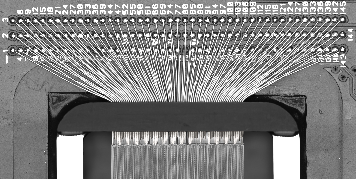
\includegraphics[width=0.85\textwidth]{files/ProbeCard}
			\caption{Top view of the probe card and its needles mounted in the probe station for testing and grading of the ASICs. The ASIC is positioned below and held in position by the vacuum plate. The needles are not yet in contact with the ASIC but are already aligned.}
			\label{im:ProbeCard}
		\end{figure}
		
		For larger ASICs such as the FASER Pre-Shower production ASIC, many more needles are required to make contact with the $\mathcal{O}(100)$ pads. For such specific applications, a custom probe-card, implementing a custom number of needles on a PCB can ne used as an interface between the ASIC and the power supplies and readout channels required for testing. Figure \ref{im:} shows the probe-card and its needles positioned on of top the ASIC's pads in the probe station. 
		While with very few needles, the alignement in all three spatial direction si performed one by one, here the alignement is constrained by two factors: the positioning and alignement of the needles on the probe card themselves; the alignement of the probe card within the frame holding it in the probe station. To ensure good electrical connection between the needles and the pads, a sufficient pressure needs to be applied. Even a very small offset, especially in the vertical direction, could compromise contact, hence affecting the quality of the testing and grading results.
		
		The grading of ASICs was performed systematically, three different grades could be assigned: \textbf{A} for ASICs following nominal behaviour, \textbf{B} for ASICs with some manageable defects and \textbf{C} for unusable ASICs. The testing procedure was identical for every ASIC and was composed of the test presented below. 
		\subsubsection{Low-Voltage and High-Voltage}
			The LV is provided to the ASIC, powering up the electronics (both analog and digital). The registers of the ASICs are configured to a standard working point, hence fixing its power consumption. The current pulled on the LV power supply was previously measured for single ASICs exhibiting good behaviour and performances, the value expected is around \SI{36}{\milli\ampere}. Any much different value could hint at defects in the ASIC, compromising its operation.
			
			Ensuring that the current pulled by the ASIC on the HV power supply allows to asses whether it exhibits the electrical behaviour of a diode in reversed-bias. Once again, the reference values for good behaviour were defined doing full IV curves, at HV = \SI{-100}{\volt} and HV = \SI{200}{\volt} the current are respectively expected to be \SI{7}{\nano\ampere} and \SI{12}{\nano\ampere}. The ASIC could exhibit an Ohmic behaviour which would be symptomatic of a defect leading to a short somewhere in the ASIC, hence making it impossible to operate properly. The ASIC could also pull a much higher current than the expected one, as long as the IV trend is not Ohmic, this is a-priori not an issue unless the current is order of magnitudes higher than the expect values, this should be taken into account when grading. The results of the tests are presented in figure \ref{im:asic_stat_HV+LV}.
			\begin{figure}[h]
				\centering
				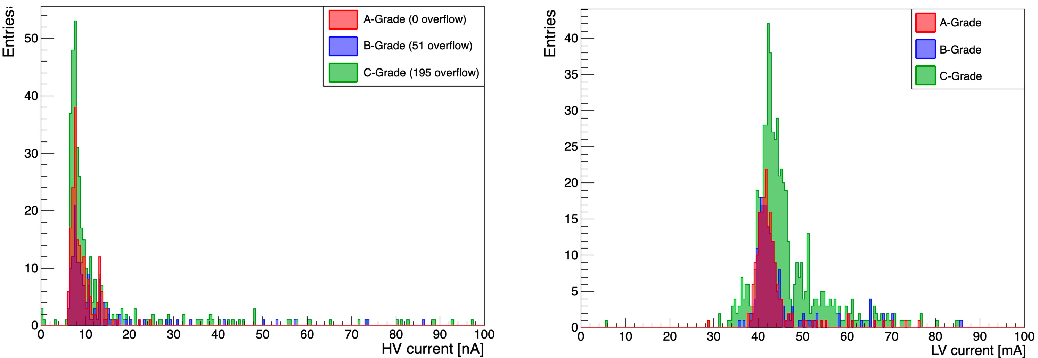
\includegraphics[width=1.0\textwidth]{files/asic_stat_HV+LV}
				\caption{Distribution of the current from the high voltage (left) and low voltage (right) power supplies, separated for the three different grades. The distribution of the HV current for \textbf{B}-grade and \textbf{C}-grade has a significant number of overflows, quoted in the legend.}
				\label{im:asic_stat_HV+LV}
			\end{figure}
			
			Only if the HV current values was in the $\mathcal{O}(10)$ nA range and the LV current was in the $\mathcal{O}(10)$ mA range, an \textbf{A}-grade would be associated to the ASIC.
			
		\subsubsection{Signal integrity}
			The quality of the signal from the data-out and clock lines is essential in determining the quality of production of an ASIC. The signals are transported by sub-LVDS lines, the nominal amplitude of the data.out is expected to be around \SI{250}{\milli\volt} such that the receiving elements on the PPB can sample properly sample the signal. 
			The phase between the clock and the data-out is also measures as it ensure that the level of the data-out signal is sampled at the correct position in time. The nominal value is expected to be, for a readout clock of \SI{25}{\mega\hertz}, around \SI{30.5}{\nano\second}, with a standard deviation of \SI{11}{\pico\second}. Only if the measured values of amplitude were \SI{200}{\milli\volt} and above, phase were within \SI{0.5}{\nano\second} of the nominal value and standard deviation not higher than \SI{20}{\pico\second}, the ASIC would receive an \textbf{A} grade. 
			Additionally, some data is collected and converted, if them aforementioned parameters are not optimal, this could lead to corrupted data, hence a failed data conversion, often leading to 100\% of the date being unusable. This is evidently a criteria automatically classifying an ASIC with a \textbf{C}-grade. 
			\begin{figure}[h]
				\centering
				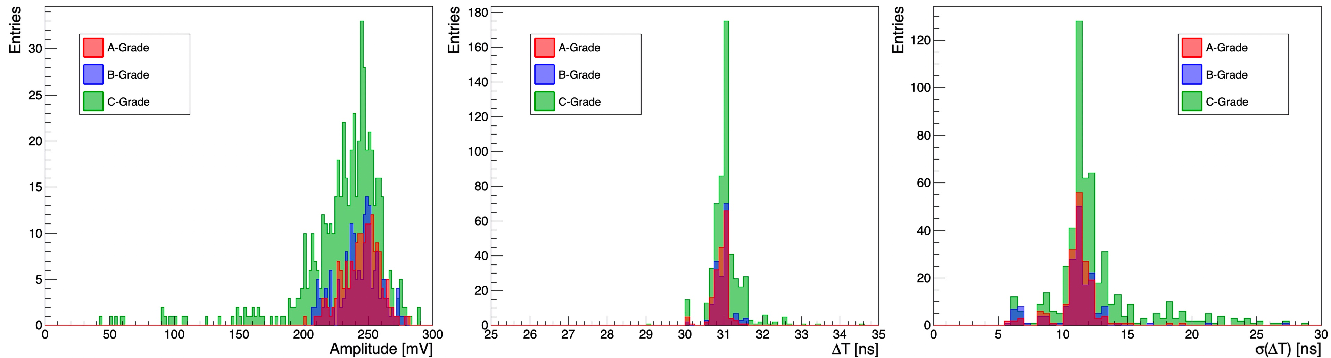
\includegraphics[width=1.0\textwidth]{files/asic_stat_signalquality}
				\caption{Distribution of the amplitude of the sub-LVDS signal for the data out line (left), time difference (or phase) between the data out signal and the read-out clock line (center) and standard deviation of the time difference (right). The distributions for the three types of gardes are overlayed. }
				\label{im:asic_stat_signalquality}
			\end{figure}
		
		\subsubsection{Digital: masking and test-pulse}
			The ASIC has to be fully maskable, meaning that it could be operated silently even if at a low operating threshold, some noisy pixels are present in the matrix. A first test is performed by setting the threshold to the lowest possible values and without injecting testpulse, followed by a test with higher threshold.
			If the masking is working as expected, none of the previous scenarios described should lead to data being read-out from the ASIC. The purpose of the second test is to understand, of some pixel were found to be noisy, if a reasonably low threshold could make them silent. If all of the ASIC could be masked, the ASIC would be graded \textbf{A}, if some structures couldn't be masked, but a reasonably higher threshold could make it silent, the garde associated would be \textbf{B}, otherwise, \textbf{C}.
			In complement, some pixels in the first four rows of each column were unmasked so that a test-pulse could also be injected in a specific pattern. The test-pulse needed to be successfully injected in all SCs such that the ASIC could receive an \textbf{A}-grade.  
		       
		       
		\subsubsection{Baseline and Threshold}
			If the ASIC was fully maskable, a single pixel was unmasked and the level of the baseline of the noise is found adjusting the values for the registers associated to $threshold\_set$ and $threshold\_offset$. Once the pixel is silent, the value is measured in mV on one of the interface board for communication and powering through the probe-card. The value is expected to be around \SI{700}{\milli\volt} for an ASIC to be classified with an \textbf{A}-grade but the value is not directly used for determining the grade. 
			
			A more meaningful test to be performed is a very coarse threshold scan, performed by unmasking the entire ASIC and by collecting data for a threshold fixed at the level of the baseline of the noise and then and then add 5 and 10 DAC values to the $threshold\_set$ register and collect data again. The expected behaviour is a decrease of the amount of noisy pixel, indicating an expected spread in noise and seeing if the threshold has an effect on the matrix or not. If the behaviour was a described above, the ASIC would receive be graded with an \textbf{A}-garde. \\
			
			
			The combined results of all of the test allowed to assign a grade to each ASIC. The proportion of \textbf{A}-grade, \textbf{B}-grade and \textbf{C}-grade ASICs is presented in the figure \ref{im:asic_grade_repartition}, along with a more detailed separation within the \textbf{C}-grade ASICs according to their behaviours.
			\begin{figure}[h]
				\centering
				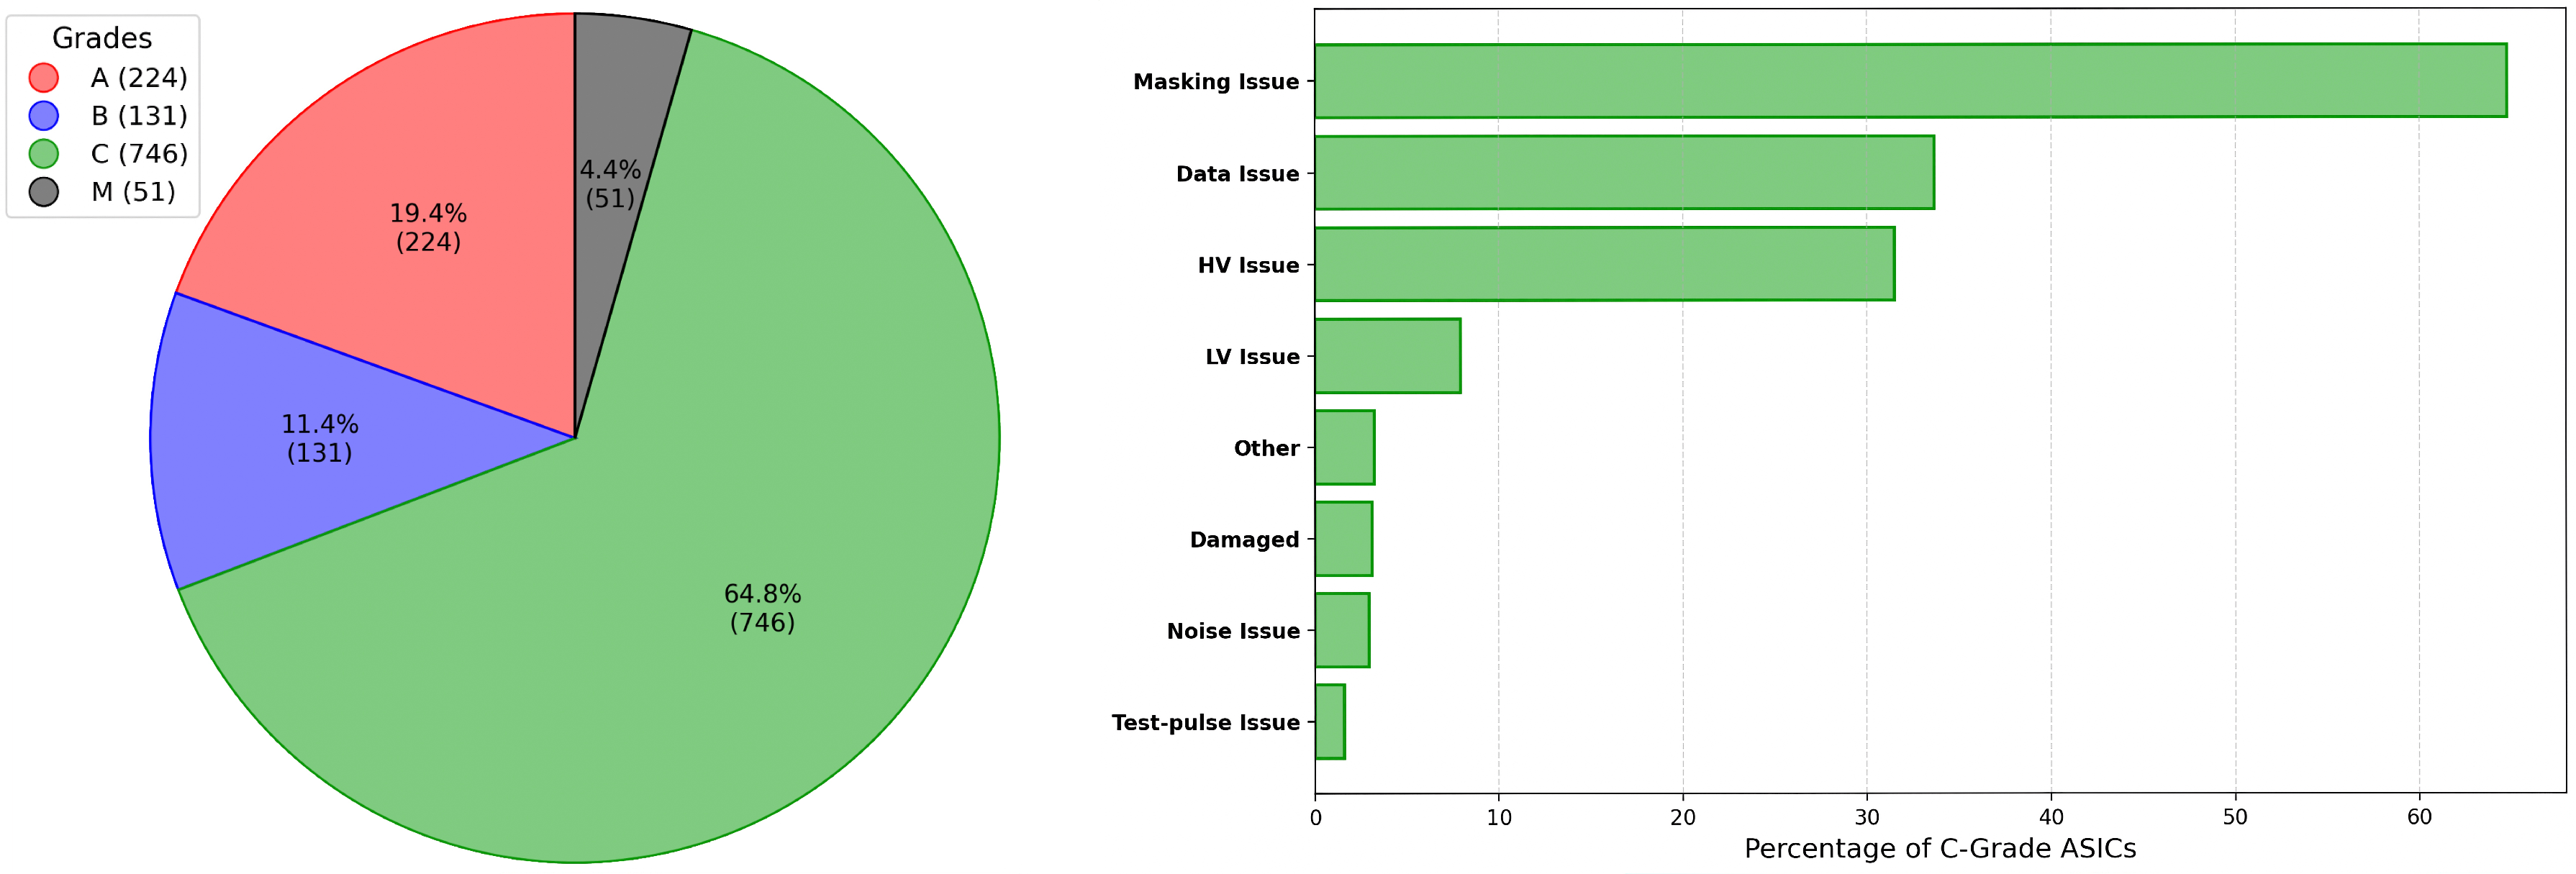
\includegraphics[width=1.0\textwidth]{files/asic_grade_repartition}
				\caption{Distribution of the garde given to the 1152 ASICs tested. An additional \textbf{M}-grade was added for missing ASICs, either damaged during the post processing procedures or exhibiting visual production defects (left). Distribution of the features of the \textbf{C}-grade ASICs (right), more than one feature can be exhibited by a single ASIC.}
				\label{im:asic_grade_repartition}
			\end{figure}
			
			The production yield can be estimated as the fraction of the total number of ASICs produced, classified as \textbf{A}-grade ASICs, hence 19.4\%. It is striking that almost 65\% of the ASICs were classified as \textbf{C}-grade, much lower than the conservative estimation made using the yield on the pre-production ASIC and scaling it accordingly to the respectives areas of the prototypes. Some thorough studies have been performed in order to identify the cause of the poor production yield, most of the ASIC exhibit issues linked to the masking of pixels, followed by issues in the data quality and issues linked to the response in current to the depletion voltage. 
			The \textbf{B}-grade ASICs shouldn't be accounted for in the production yield but should rather be taken into account in the defective ASICs. Since the delivery of at least 4 detector planes (288 ASICs assuming a 100\% module production yield) was essential for the performances of the entire Pre-Shower detector, a sub-classification of \textbf{B}-grade ASICs was performed in order to select the ones with least defects and gradually assemble them on modules. 
			
			 It is important to recall that designing such large ASICs is far from trivial and with the very strict deadlines on the project combined to the delays in delivery of the pre-production prototype, a production yield of almost 20\% is not to be underestimated, although not complying entirely with the requirement of the project. 
			 \clearpage
			
		
		\subsection{Module assembly \textcolor{red}{ 3 pages}}
		
		The assembly of 6 ASICs within a module is of critical importance as it may impact the overall performance of the detector. It was discussed before that the module is in charge of establishing both powering and communication between the ASICs and the readout and control system. It also couples thermally the ASICs to the cooling system, maintaining them at a constant operational temperature and provide support for alignement of the ASICs among themselves, aiming at the minimal additional dead-area in the detector, due to poor positioning of the ASICs. 
		
		The assembly procedure can be broken down into 4 successive steps for which the different trials along with measurements and the final procedure, will be presented.  
			\subsubsection{Alignement of ASICs}
			The 6 selected ASICs for assembly in a module has first to be cleaned using a plasma machine, ensuring no potential contamination by dust which could present a potential flaw in terms of mechanical integrity. The ASICs are ten positioned in a 3$\times$2 array, with the digital and I/O periphery facing outward. A plastic L-shaped tool is used to perform the alignement by blocking the ASICs in the top corner of the top assembly frame. Once the ASICs are in position, a gentle suction is performed thanks to holes drilled in the assembly frame so that the ASICs can be held in position while being manipulated. Figure \ref{im:module_assembly_0} shows the alignement of the ASICs onto the top assembly frame. 
			\begin{figure}[h]
				\centering 
				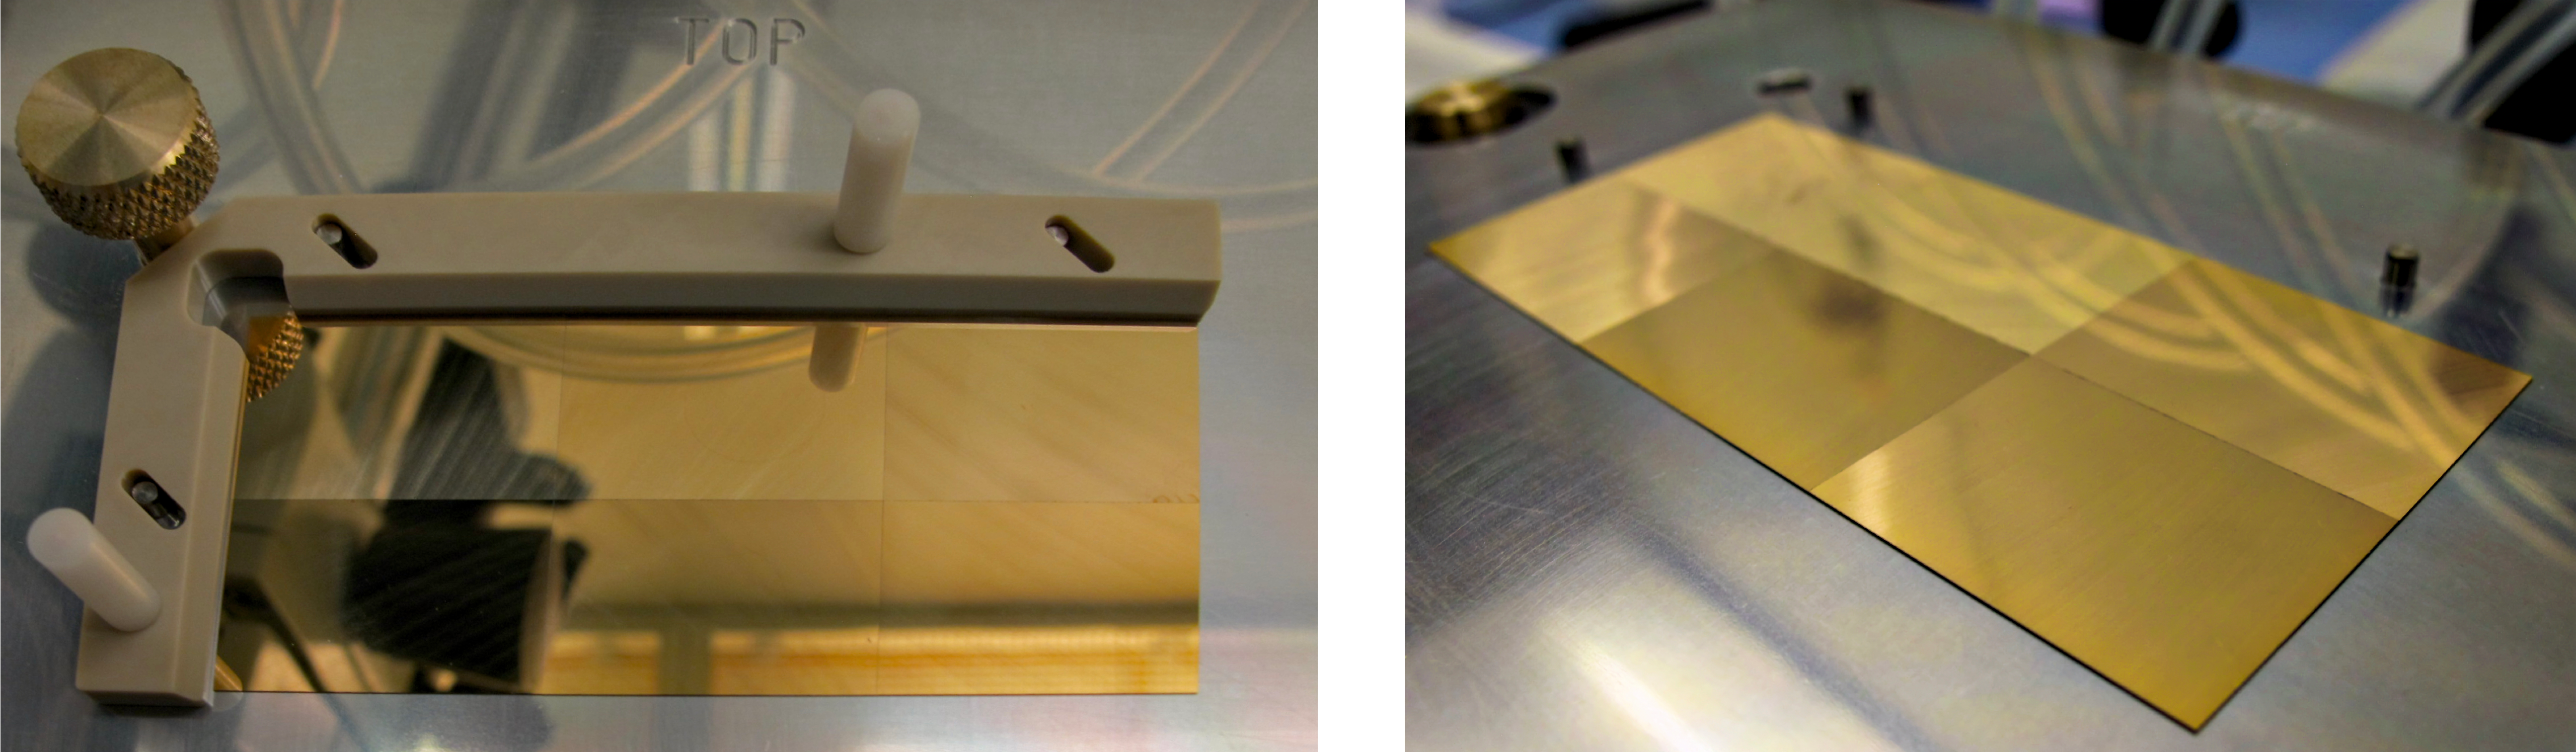
\includegraphics[width=1.0\linewidth]{files/module_assembly_0}
				\caption{Alignement of the 6 ASICS into a 3$\times$2 array using the L-shaped plastic tool (left) and later held into position using vacuum through drilled holes within the top assembly frame (right)}
				\label{im:module_assembly_0} 
			\end{figure}
			
			\subsubsection{Glueing on base-plate}
			At first, the glue was deposited using a tool instrumented with a sponge at its end, absorbing the glue and depositing it evenly on the surface of the base plate. Even if this technique provided a good and even spread of the glue, there was not control on the thickness of glue deposited, resulting in modules being assembled with an insufficient amount of glue and ASICs consequently detaching from the surface of the base plate.
			
			A refined procedure defined, implementing the deposition of a thin layer of glue being deposited on top of the base plates using \SI{150}{\micro\meter}-thick metallic frame, constraining the thickness of glue to a sufficient amount. The glue is evenly spread using a plastic spatula and a fixed number of back and forth mouvement across the length of the module. The metallic frame is shaped such that it avoids glue deposition in the interstices separating the ASIC and at the edges of the base plate. This later detail in glue deposition will be relevant for a later discussion.   
			
			The glue chosen was first an Araldyte glue mixed together with small aluminium balls to provide better thermal coupling but later was changed to Araldyte glue without any aluminium balls as it was identified with an issue in HV current causing the current to drift over time towards high values, couple order of magnitudes higher than the expected values from probe station measurements. Figure \ref{im:module_assembly_1bis} shows the ASICs held in position on the top assembly frame and the bottom assembly frame with the metallic plate mounted on the base-plate and the glue deposited on top of it. 
			\begin{figure}[h]
				\centering 
				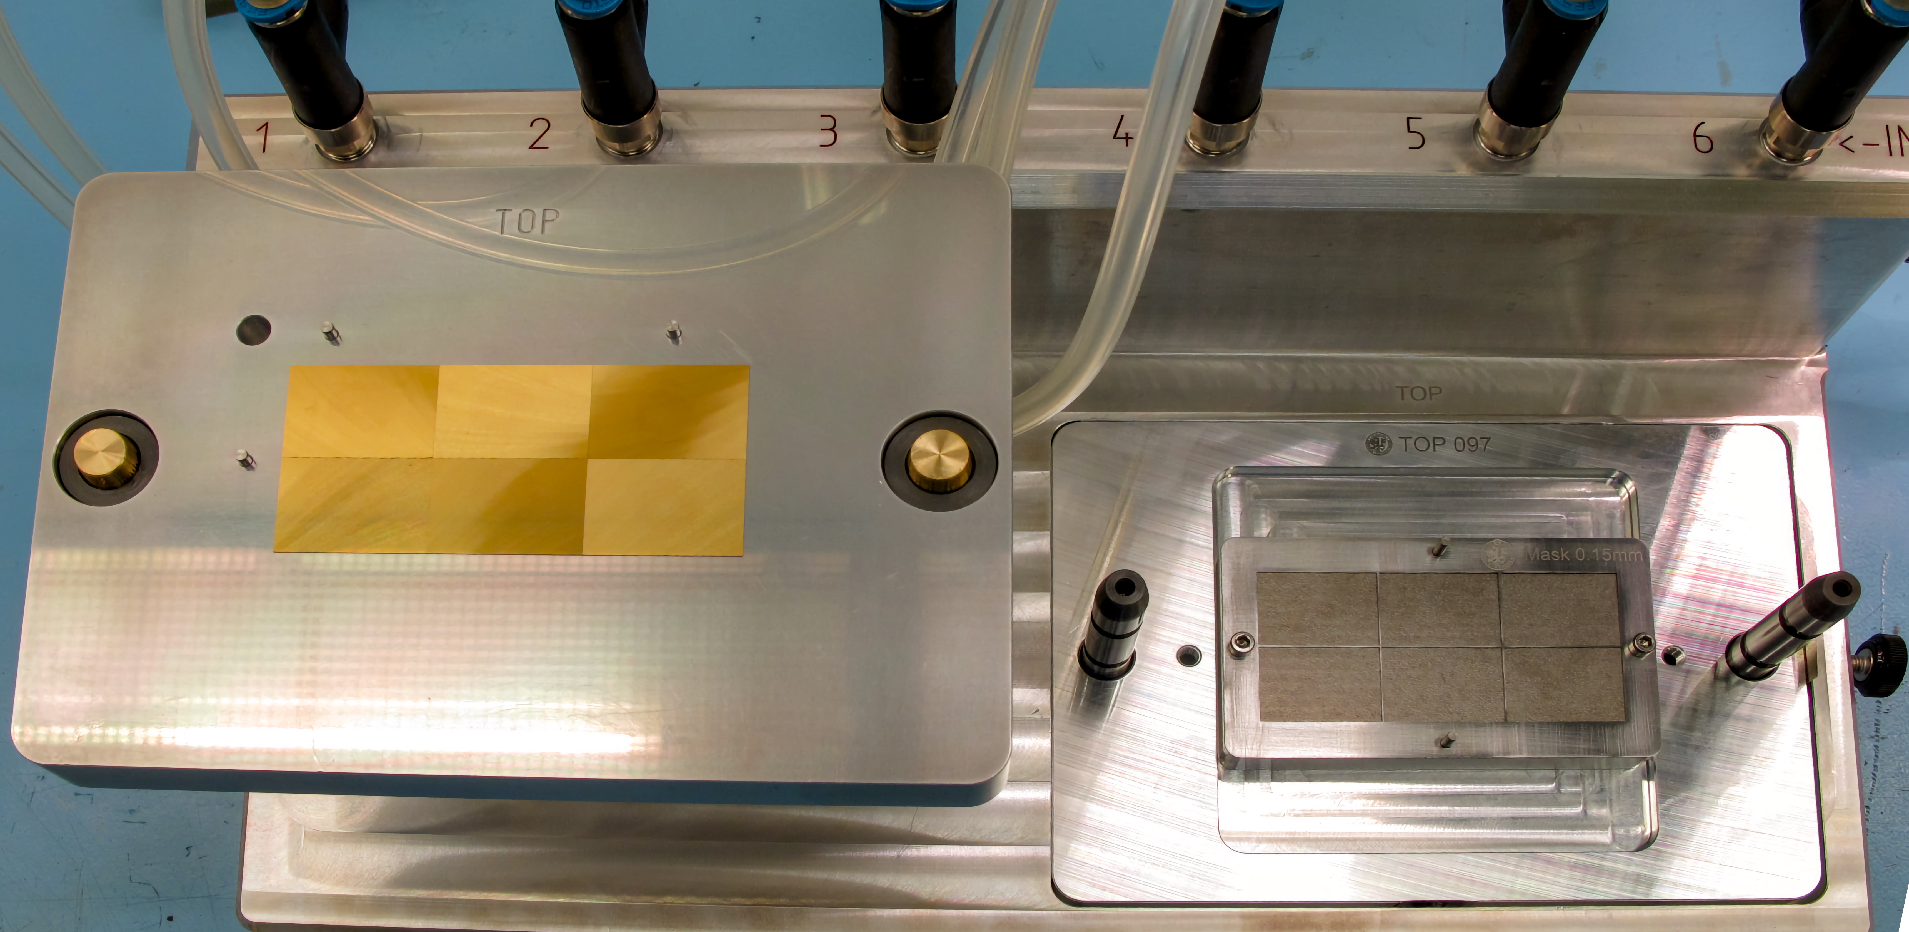
\includegraphics[width=0.8\linewidth]{files/module_assembly_1bis}
				\caption{Preparation of glueing of the 6 ASICs on top of the base plate after the deposition of a \SI{150}{\micro\meter}-thick layer of glue across the entire base-plate surface at the exception of the edges of the modules and the interstices between the ASICs.}
				\label{im:module_assembly_1bis} 
			\end{figure}
			
			Once the glue was deposited, the top assembly frame is precisely aligned using the alignement pillars as can be seen on the right of figure \ref{im:module_assembly_1bis}. Once in contact, a pressure equivalent to a weight of \SI{500}{\gram} will be applied to ensure optimal contact between the ASIC and the glue on the base-plate. 
			At first, the vacuum was held during the drying of the glue to make sure the ASICs would not move during the process. This technique was accompanied with a series of assembly failures during which the glue would infiltrate through capillarity in-between the ASICs and on the edges of the module due to the suction power of the vacuum holding in position the ASICs. This resulted in ASICs being glued to the top assembly frame too, hence making it very dangerous to remove the frame, sometimes resulting, like in the case of module \textit{ELECT07} in the peeling of some layers of the ASICs, exposing its internal structures and damaging it to a point of no return, as shown in Figure \ref{im:module_assembly_fail}. 
			\begin{figure}[h]
				\centering 
				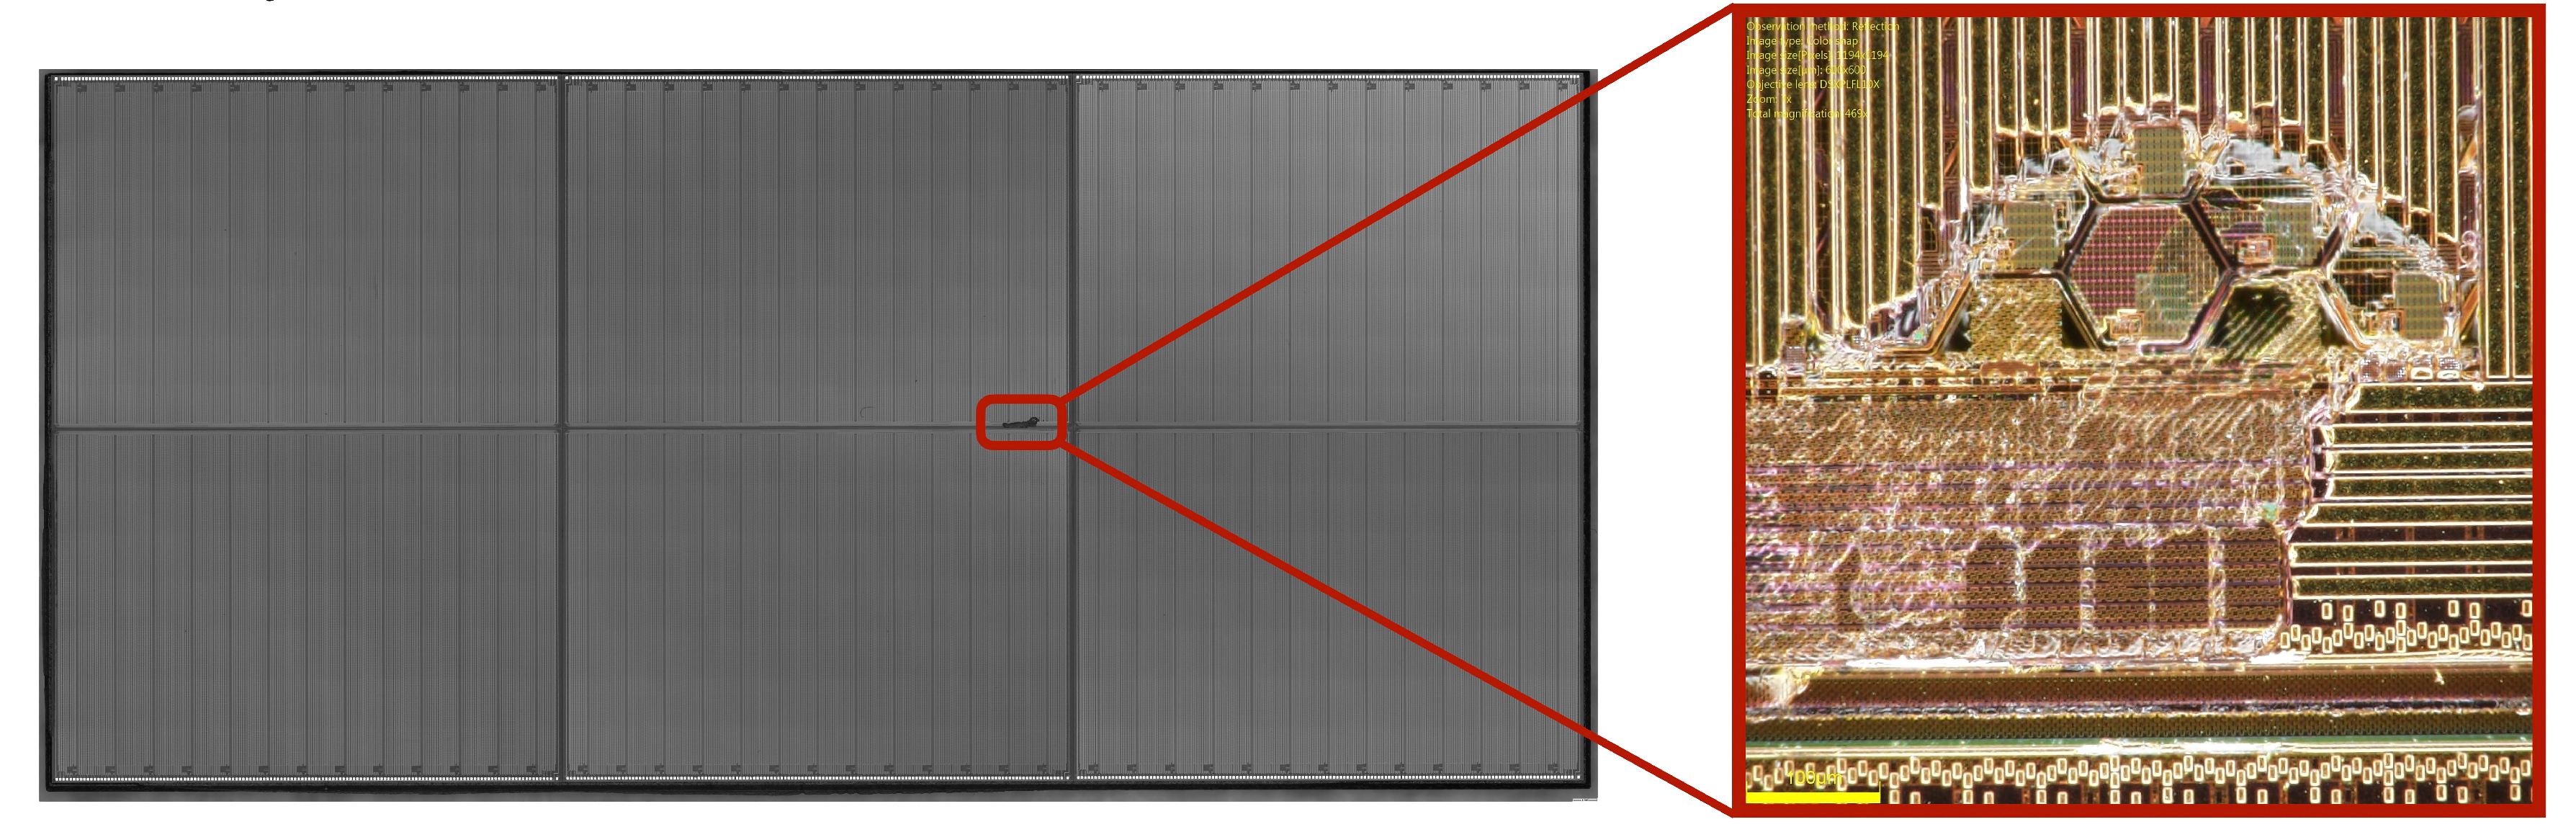
\includegraphics[width=1.0\linewidth]{files/module_assembly_fail}
				\caption{Assembly failure for which glue infiltrated into the interstice between ASICs at the center of the module. This resulted in ASIC 2 being pealed from its upper metal layers, unveiling the hexagonal pixels of the matrix and their front-end electronics.}
				\label{im:module_assembly_fail} 
			\end{figure}
			
			The final procedure was adapted and the vacuum was removed while the glue was drying. Additional care was taken by limiting the deposition of glue in the regions below the interstices between ASICs to disfavour even more the infiltration of glue. A deviation of the ASICs from the aligned position was expected but measured to be below \SI{100}{\micro\meter} in the worst cases. Evidently, any loss at the level of the modules, even of a single ASIC, becomes a 6-ASIC loss as it is impossible to substitute a faulty ASIC once assembled on a module. 
			
			\subsubsection{Glueing of module-flex}
			The module-flex is glued on top of the ASICs following a similar procedure. The module flex is positioned in a second top assembly frame, aligned through the use of a precise plastic frame, using the two holes at the center of the left and right edges as reference, and held in position with vacuum. 
			
			At first, the glue was deposited homogeneously using the tool instrumented with the sponge at its end but this first procedure lead to some electrical issues. Usually, a module is expected to pull current on the HV power supply at a level compatible the sum of the individual currents for every ASIC, i.e. in the order of \SI{45}{\nano\ampere} for a depletion voltage of \SI{120}{\volt}. It was observed that some modules would pull currents at the level of \SI{1.5}{\micro\ampere}, only at a depletion voltage of \SI{2.4}{\volt}. This enormous current consumption was also associated to the unmasking of a some specific SP in a specific SC in a specific ASIC. 
			
			After reconstructing the position of the pixels responsible for this problem, it was identified to coincide with the position of the HV via in the module-flex, crossing all of its layer from the top surface to thee bottom, distributing the HV to all ASICs. This via hence needed to be insulated from the surface of the ASIC in order to avoid electrical coupling between the ASICs and the HV-via. A \SI{50}{\micro\meter}.thick layer of transparent kapton-tape was added at the location of the via and equivalently at the other side of the module to avoid mechanical constraints on the module-flex. Figure \ref{im:module_assembly_fix0} shows the glue and kapton tape applied at the bottom of the module-flex.
			\begin{figure}[h]
				\centering 
				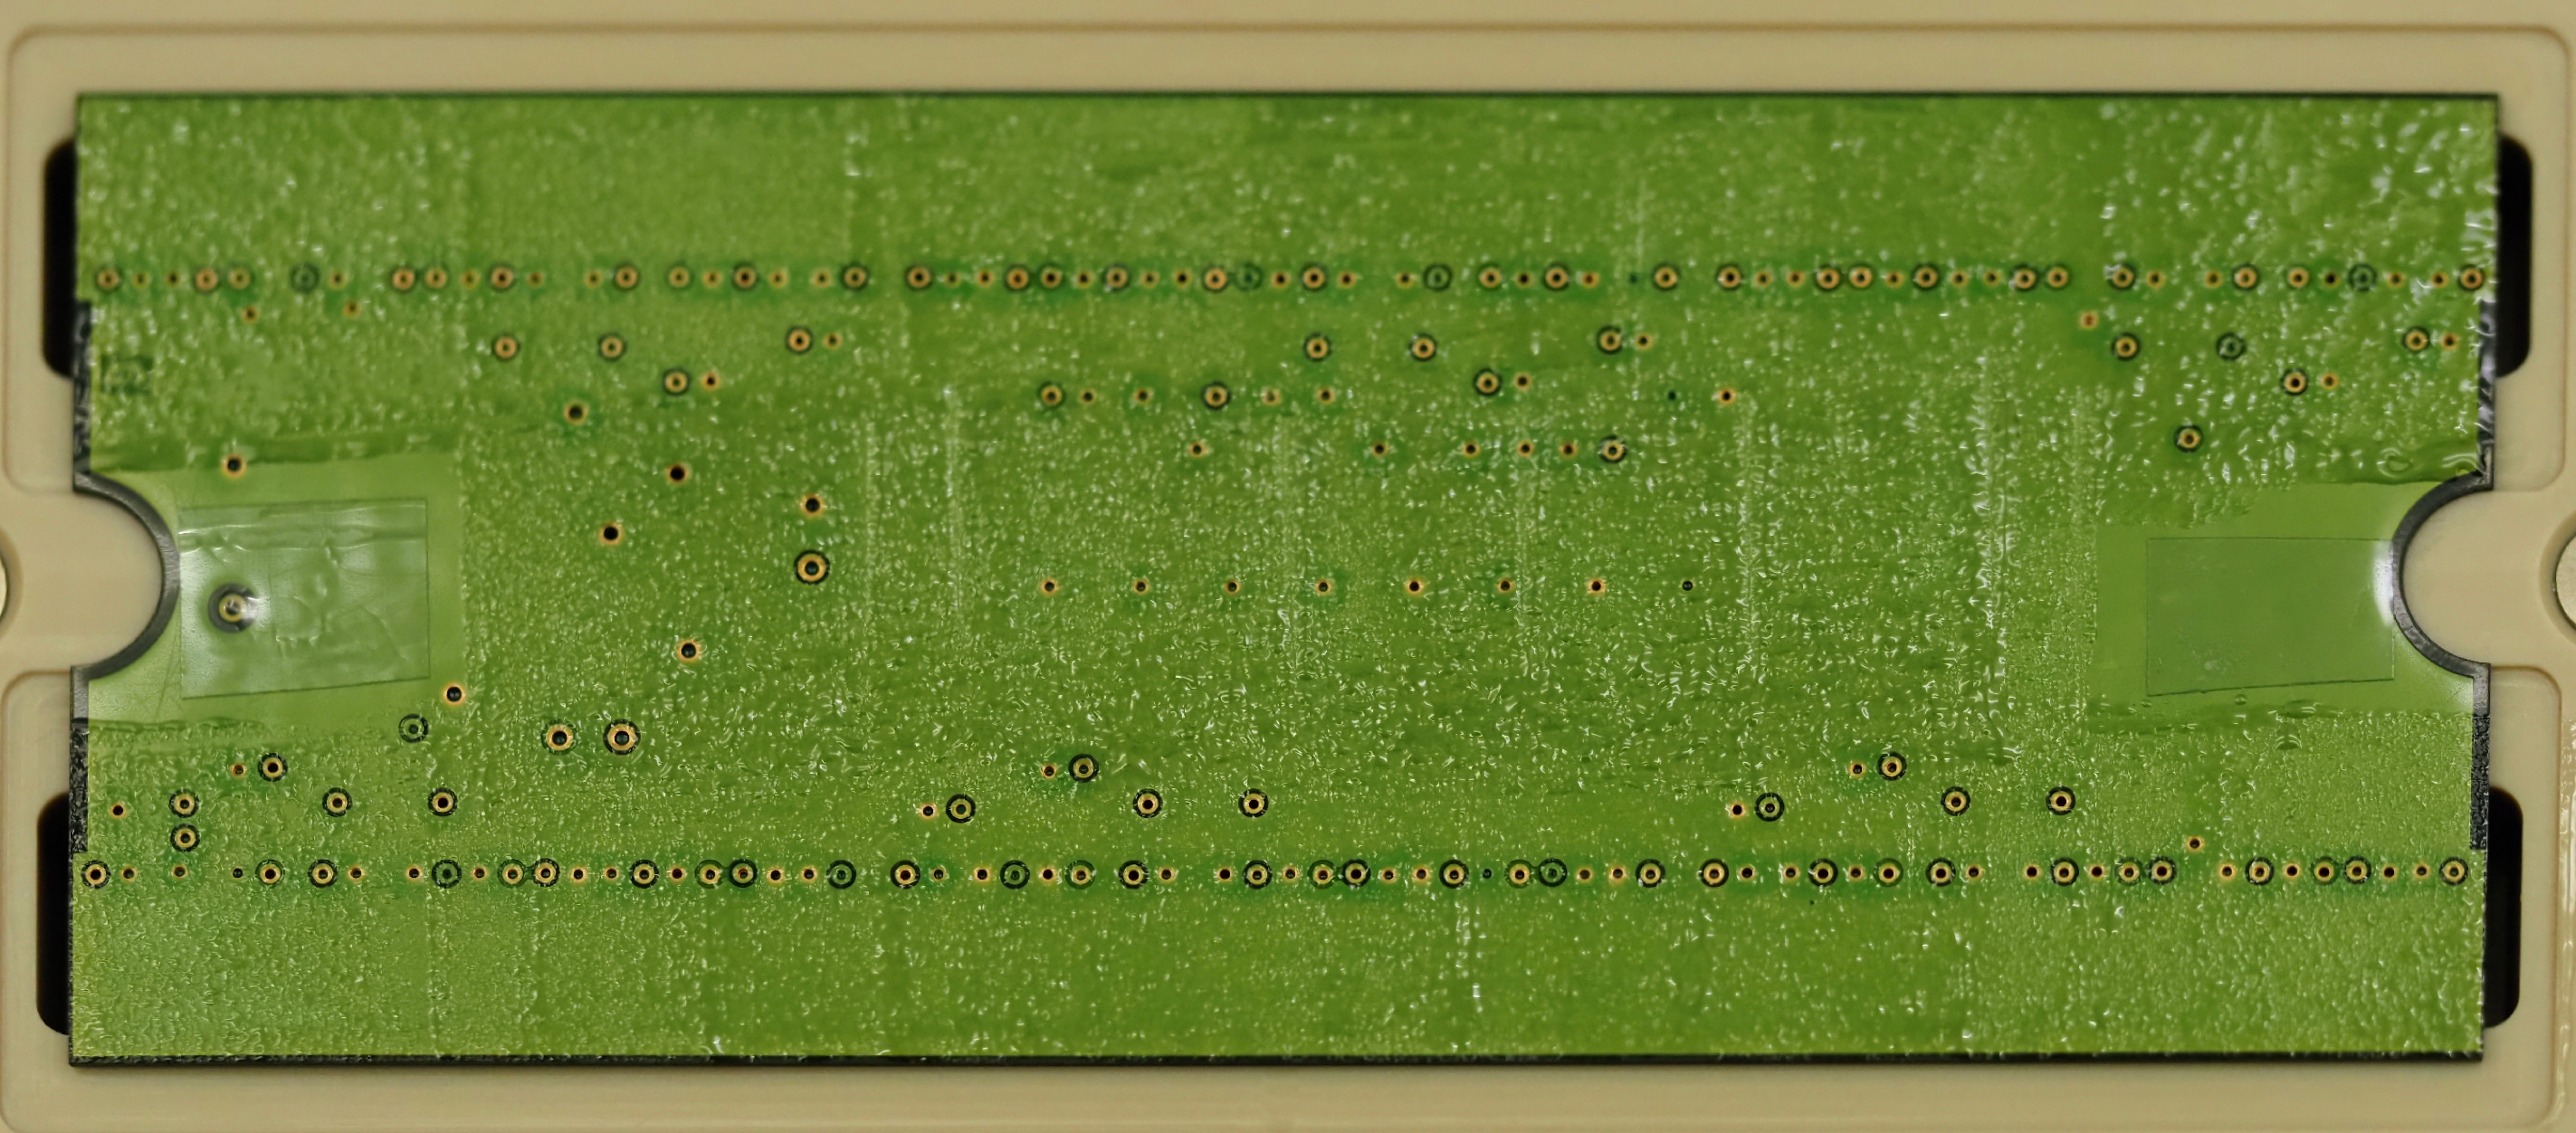
\includegraphics[width=0.7\linewidth]{files/module_assembly_fix0}
				\caption{Deposition of glue on the bottom of the module flex. On the left side, a circular HV-via goes from the top of the module-flex to the bottom, hence impacting the stability of the ASIC located underneath. A \SI{50}{\micro\meter}-thick kapton tape layer is added to electrically insulate the HV-via. An equivalent thickness of kapton tape is added at the opposite side. }
				\label{im:module_assembly_fix0} 
			\end{figure}
			
			The module flex is then aligned in position onto the ASICs using the same alignement pillars as previously, hence ensuring optimal mechanical alignement between the layers. A pressure equivalent to the weight of \SI{500}{\gram} is applied for optimal glueing. 
			Once the glue has dried, the top assembly frame can be removed and the mechanical part of the assembly procedure is finished.
			 
			\subsubsection{Wire-bonding}
			The final step of the module assembly is the electrical connection between the module-flex and the pads on the ASICs for powering and I/O. As previously mentioned, each ASIC has a total of 134 pads requiring wire-bonding, so a total of 804 wire-bonds at the level of the module. The wire bonding is, after several manual attempts to define the procedure, automatised so that, without the need of any intervention, the wire-bonding of an entire module can be performed in under \SI{20}{\minute}. The presence of a technician is fondamental during this procedure as it requires extreme attention to control the quality of the wire-bonds. Some are specifically difficult to do and have to be manually performed in some cases, requiring great precision and care to avoid damaging neighbouring wire-bonds or components. The wire-bonding machines produces the electrical connection through supersonic waves, melting the tip of the very thin wire onto the pads on both ends through the application of a precisely calibrated pressure. Figure \ref{im:bonding} shows a module after wire-bonding was performed. 
			
			\begin{figure}[h]
				\centering 
				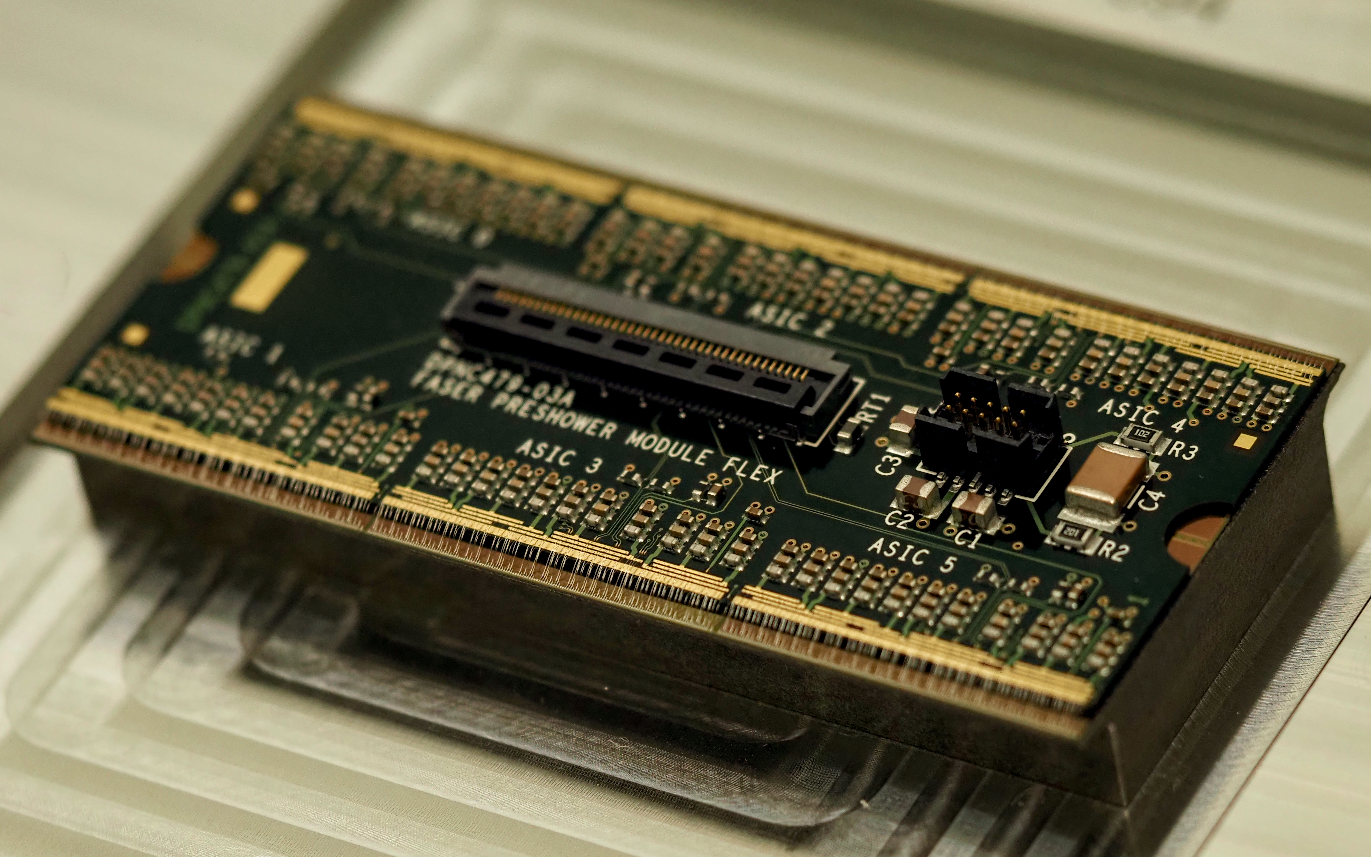
\includegraphics[width=0.7\linewidth]{files/bonding}
				\caption{Wire-bonding between a module-flex and the pads of the ASIC located underneath. T}
				\label{im:bonding} 
			\end{figure}
			
		
		
		
		
		
		
		
		
% TODO: Test with different glues, solidity and current, show the effect of dry air on the glue, show the chip getting unglued etc. Very difficult procedure  

		\subsection{Characterisation set-up \textcolor{red}{ 3 pages}}
% TODO: Show the two set-ups with the cooling plates, APP, LB power supplies and oscilloscope explain what needs to be followed carefully, currents. etc. etc.

		\subsection{Front-End working points \textcolor{red}{ 2 pages}}	
% TODO: Explain how two working point are needed for the different planes and how the different working points were defined, explain that all of the test had to be done for these two working points. Minimal sensitivity to a certain TP value. 
		
		\subsection{Threshold and Noise scans \textcolor{red}{ 4 pages}}
% TODO: Plot of the distribution of the threshold value for all the ASIC, also show at the threshold what is the amount of problematic pixels. 
% TODO: Distribution of the sigma_V extracted from the S curves. 
% TODO: Map at the level of the ASICs of the problematic pixels 
% TODO: Map at the level of the module of the problematic pixels. 
% TODO: On the noise scan, see if there is a correlation with the position == The Maps. 
		
		\subsection{Load scan and Charge calibration \textcolor{red}{ 4 pages}} 
% TODO: Explain the procedure  
		
		\subsection{Plane assembly \textcolor{red}{ 3 pages}}
% TODO: Show the mapping of the planes and how it was made from the testpulse scan plots and using the thresholds 
% TODO: Show the noisy pixels maps for the full plane. 	
	
	
	
	
	
	\clearpage
	\section{Trigger and Data Acquisition: TDAQ \textcolor{blue}{ 9 pages}}
		\subsection{Readout\textcolor{red}{ 2 pages}}
% TODO: Done already in previous chapter, is it enough ?
		\subsection{Data conversion \textcolor{red}{ 3 pages}}
% TODO: Not sure what to say here expect how the events are structured ? Maybe should go in the previous chapter
		\subsection{Data corruption and solutions  \textcolor{red}{ 3 pages}}
% TODO: Show the studies done with the termination of the sub-LVDS lines at 100 Ohm nominal and how it changed. 
		
	
	
	
	\clearpage
	\section{Testbeam campaign for detector commissioning}
% TODO: Describe layout with powering, trigger etc, 
% TODO: Show the beam profil, meaning that the full system was able to acquire this much data. 
% TODO - Analysis: align the preshower planes among themselves. Use the tracker information to extrapolate the position on the PreShower and clean the event displays and the future analysis I do. 
% TODO - Analysis: Show the deposited charge per plane and show there is a correlation on the position of the hits per plane. 
% TODO - Analysis: Show the energy deposited per plane per event as a function of the beam energy. 
		
		
		
		
		
		
		
		
		
		
		
		
		
		
		
		
		
		
		
		
		
		
		
		
		
		
		
		
		
		
		
		
		
		
		
		
		
		
		
		
		
		
		
		
		
		
		
		
		
		
		
		
		
		
		
		
		
		
		
		
%	\section{Pre-Production ASIC characterization \textcolor{blue}{ 6 pages}}
%		\subsection{ASIC description \textcolor{red}{ 3 pages}} 
%		\subsection{Time-Over-Threshold mismatch \textcolor{red}{ 3 pages}}